% Options for packages loaded elsewhere
\PassOptionsToPackage{unicode}{hyperref}
\PassOptionsToPackage{hyphens}{url}
%
\documentclass[
]{article}
\usepackage{lmodern}
\usepackage{amssymb,amsmath}
\usepackage{ifxetex,ifluatex}
\ifnum 0\ifxetex 1\fi\ifluatex 1\fi=0 % if pdftex
  \usepackage[T1]{fontenc}
  \usepackage[utf8]{inputenc}
  \usepackage{textcomp} % provide euro and other symbols
\else % if luatex or xetex
  \usepackage{unicode-math}
  \defaultfontfeatures{Scale=MatchLowercase}
  \defaultfontfeatures[\rmfamily]{Ligatures=TeX,Scale=1}
\fi
% Use upquote if available, for straight quotes in verbatim environments
\IfFileExists{upquote.sty}{\usepackage{upquote}}{}
\IfFileExists{microtype.sty}{% use microtype if available
  \usepackage[]{microtype}
  \UseMicrotypeSet[protrusion]{basicmath} % disable protrusion for tt fonts
}{}
\makeatletter
\@ifundefined{KOMAClassName}{% if non-KOMA class
  \IfFileExists{parskip.sty}{%
    \usepackage{parskip}
  }{% else
    \setlength{\parindent}{0pt}
    \setlength{\parskip}{6pt plus 2pt minus 1pt}}
}{% if KOMA class
  \KOMAoptions{parskip=half}}
\makeatother
\usepackage{xcolor}
\IfFileExists{xurl.sty}{\usepackage{xurl}}{} % add URL line breaks if available
\IfFileExists{bookmark.sty}{\usepackage{bookmark}}{\usepackage{hyperref}}
\hypersetup{
  pdftitle={Lab4},
  pdfauthor={Irimie Fabio},
  hidelinks,
  pdfcreator={LaTeX via pandoc}}
\urlstyle{same} % disable monospaced font for URLs
\usepackage[margin=1in]{geometry}
\usepackage{color}
\usepackage{fancyvrb}
\newcommand{\VerbBar}{|}
\newcommand{\VERB}{\Verb[commandchars=\\\{\}]}
\DefineVerbatimEnvironment{Highlighting}{Verbatim}{commandchars=\\\{\}}
% Add ',fontsize=\small' for more characters per line
\usepackage{framed}
\definecolor{shadecolor}{RGB}{248,248,248}
\newenvironment{Shaded}{\begin{snugshade}}{\end{snugshade}}
\newcommand{\AlertTok}[1]{\textcolor[rgb]{0.94,0.16,0.16}{#1}}
\newcommand{\AnnotationTok}[1]{\textcolor[rgb]{0.56,0.35,0.01}{\textbf{\textit{#1}}}}
\newcommand{\AttributeTok}[1]{\textcolor[rgb]{0.77,0.63,0.00}{#1}}
\newcommand{\BaseNTok}[1]{\textcolor[rgb]{0.00,0.00,0.81}{#1}}
\newcommand{\BuiltInTok}[1]{#1}
\newcommand{\CharTok}[1]{\textcolor[rgb]{0.31,0.60,0.02}{#1}}
\newcommand{\CommentTok}[1]{\textcolor[rgb]{0.56,0.35,0.01}{\textit{#1}}}
\newcommand{\CommentVarTok}[1]{\textcolor[rgb]{0.56,0.35,0.01}{\textbf{\textit{#1}}}}
\newcommand{\ConstantTok}[1]{\textcolor[rgb]{0.00,0.00,0.00}{#1}}
\newcommand{\ControlFlowTok}[1]{\textcolor[rgb]{0.13,0.29,0.53}{\textbf{#1}}}
\newcommand{\DataTypeTok}[1]{\textcolor[rgb]{0.13,0.29,0.53}{#1}}
\newcommand{\DecValTok}[1]{\textcolor[rgb]{0.00,0.00,0.81}{#1}}
\newcommand{\DocumentationTok}[1]{\textcolor[rgb]{0.56,0.35,0.01}{\textbf{\textit{#1}}}}
\newcommand{\ErrorTok}[1]{\textcolor[rgb]{0.64,0.00,0.00}{\textbf{#1}}}
\newcommand{\ExtensionTok}[1]{#1}
\newcommand{\FloatTok}[1]{\textcolor[rgb]{0.00,0.00,0.81}{#1}}
\newcommand{\FunctionTok}[1]{\textcolor[rgb]{0.00,0.00,0.00}{#1}}
\newcommand{\ImportTok}[1]{#1}
\newcommand{\InformationTok}[1]{\textcolor[rgb]{0.56,0.35,0.01}{\textbf{\textit{#1}}}}
\newcommand{\KeywordTok}[1]{\textcolor[rgb]{0.13,0.29,0.53}{\textbf{#1}}}
\newcommand{\NormalTok}[1]{#1}
\newcommand{\OperatorTok}[1]{\textcolor[rgb]{0.81,0.36,0.00}{\textbf{#1}}}
\newcommand{\OtherTok}[1]{\textcolor[rgb]{0.56,0.35,0.01}{#1}}
\newcommand{\PreprocessorTok}[1]{\textcolor[rgb]{0.56,0.35,0.01}{\textit{#1}}}
\newcommand{\RegionMarkerTok}[1]{#1}
\newcommand{\SpecialCharTok}[1]{\textcolor[rgb]{0.00,0.00,0.00}{#1}}
\newcommand{\SpecialStringTok}[1]{\textcolor[rgb]{0.31,0.60,0.02}{#1}}
\newcommand{\StringTok}[1]{\textcolor[rgb]{0.31,0.60,0.02}{#1}}
\newcommand{\VariableTok}[1]{\textcolor[rgb]{0.00,0.00,0.00}{#1}}
\newcommand{\VerbatimStringTok}[1]{\textcolor[rgb]{0.31,0.60,0.02}{#1}}
\newcommand{\WarningTok}[1]{\textcolor[rgb]{0.56,0.35,0.01}{\textbf{\textit{#1}}}}
\usepackage{graphicx}
\makeatletter
\def\maxwidth{\ifdim\Gin@nat@width>\linewidth\linewidth\else\Gin@nat@width\fi}
\def\maxheight{\ifdim\Gin@nat@height>\textheight\textheight\else\Gin@nat@height\fi}
\makeatother
% Scale images if necessary, so that they will not overflow the page
% margins by default, and it is still possible to overwrite the defaults
% using explicit options in \includegraphics[width, height, ...]{}
\setkeys{Gin}{width=\maxwidth,height=\maxheight,keepaspectratio}
% Set default figure placement to htbp
\makeatletter
\def\fps@figure{htbp}
\makeatother
\setlength{\emergencystretch}{3em} % prevent overfull lines
\providecommand{\tightlist}{%
  \setlength{\itemsep}{0pt}\setlength{\parskip}{0pt}}
\setcounter{secnumdepth}{-\maxdimen} % remove section numbering

\title{Lab4}
\usepackage{etoolbox}
\makeatletter
\providecommand{\subtitle}[1]{% add subtitle to \maketitle
  \apptocmd{\@title}{\par {\large #1 \par}}{}{}
}
\makeatother
\subtitle{Exercises}
\author{Irimie Fabio}
\date{}

\begin{document}
\maketitle

{
\setcounter{tocdepth}{2}
\tableofcontents
}
\hypertarget{exercise-1}{%
\section{Exercise 1}\label{exercise-1}}

\hypertarget{a}{%
\subsection{A}\label{a}}

Plot the Probability Mass Function for the Binomial distribution with
\(n=18\) and \(p=\frac{1}{3}\). Calculate:

\begin{enumerate}
\def\labelenumi{\arabic{enumi}.}
\tightlist
\item
  \(P(X=3)\)
\end{enumerate}

\begin{Shaded}
\begin{Highlighting}[]
\KeywordTok{dbinom}\NormalTok{(}\DecValTok{3}\NormalTok{, }\DecValTok{18}\NormalTok{, }\DecValTok{1} \OperatorTok{/}\StringTok{ }\DecValTok{3}\NormalTok{)}
\CommentTok{\#\# [1] 0.06901723}
\end{Highlighting}
\end{Shaded}

\begin{enumerate}
\def\labelenumi{\arabic{enumi}.}
\setcounter{enumi}{1}
\tightlist
\item
  \(P(X \ge 3)\)
\end{enumerate}

\begin{Shaded}
\begin{Highlighting}[]
\DecValTok{1} \OperatorTok{{-}}\StringTok{ }\KeywordTok{pbinom}\NormalTok{(}\DecValTok{2}\NormalTok{, }\DecValTok{18}\NormalTok{, }\DecValTok{1} \OperatorTok{/}\StringTok{ }\DecValTok{3}\NormalTok{)}
\CommentTok{\#\# [1] 0.9673521}
\CommentTok{\# or}
\KeywordTok{pbinom}\NormalTok{(}\DecValTok{2}\NormalTok{, }\DecValTok{18}\NormalTok{, }\DecValTok{1} \OperatorTok{/}\StringTok{ }\DecValTok{3}\NormalTok{, }\DataTypeTok{lower.tail =} \OtherTok{FALSE}\NormalTok{)}
\CommentTok{\#\# [1] 0.9673521}
\end{Highlighting}
\end{Shaded}

\begin{enumerate}
\def\labelenumi{\arabic{enumi}.}
\setcounter{enumi}{2}
\tightlist
\item
  \(P(1 \le X < 5)\)
\end{enumerate}

\begin{Shaded}
\begin{Highlighting}[]
\KeywordTok{pbinom}\NormalTok{(}\DecValTok{4}\NormalTok{, }\DecValTok{18}\NormalTok{, }\DecValTok{1} \OperatorTok{/}\StringTok{ }\DecValTok{3}\NormalTok{) }\OperatorTok{{-}}\StringTok{ }\KeywordTok{pbinom}\NormalTok{(}\DecValTok{0}\NormalTok{, }\DecValTok{18}\NormalTok{, }\DecValTok{1} \OperatorTok{/}\StringTok{ }\DecValTok{3}\NormalTok{)}
\CommentTok{\#\# [1] 0.2303957}
\end{Highlighting}
\end{Shaded}

\begin{enumerate}
\def\labelenumi{\arabic{enumi}.}
\setcounter{enumi}{3}
\tightlist
\item
  \(P(X \ge 15)\)
\end{enumerate}

\begin{Shaded}
\begin{Highlighting}[]
\KeywordTok{pbinom}\NormalTok{(}\DecValTok{14}\NormalTok{, }\DecValTok{18}\NormalTok{, }\DecValTok{1} \OperatorTok{/}\StringTok{ }\DecValTok{3}\NormalTok{, }\DataTypeTok{lower.tail =} \OtherTok{FALSE}\NormalTok{)}
\CommentTok{\#\# [1] 1.852509e{-}05}
\end{Highlighting}
\end{Shaded}

\begin{Shaded}
\begin{Highlighting}[]
\KeywordTok{library}\NormalTok{(ggplot2)}
\NormalTok{df \textless{}{-}}\StringTok{ }\KeywordTok{data.frame}\NormalTok{(}\DataTypeTok{x =} \DecValTok{0}\OperatorTok{:}\DecValTok{18}\NormalTok{, }\DataTypeTok{y =} \KeywordTok{dbinom}\NormalTok{(}\DecValTok{0}\OperatorTok{:}\DecValTok{18}\NormalTok{, }\DecValTok{18}\NormalTok{, }\DecValTok{1} \OperatorTok{/}\StringTok{ }\DecValTok{3}\NormalTok{))}

\KeywordTok{ggplot}\NormalTok{(df, }\KeywordTok{aes}\NormalTok{(}\DataTypeTok{x =}\NormalTok{ x, }\DataTypeTok{y =}\NormalTok{ y, }\DataTypeTok{fill =} \StringTok{"PMF"}\NormalTok{)) }\OperatorTok{+}
\StringTok{  }\KeywordTok{geom\_col}\NormalTok{() }\OperatorTok{+}
\StringTok{  }\KeywordTok{scale\_x\_continuous}\NormalTok{(}\DataTypeTok{breaks =} \DecValTok{0}\OperatorTok{:}\DecValTok{18}\NormalTok{) }\OperatorTok{+}
\StringTok{  }\KeywordTok{scale\_fill\_manual}\NormalTok{(}\DataTypeTok{values =} \StringTok{"red"}\NormalTok{) }\OperatorTok{+}
\StringTok{  }\KeywordTok{labs}\NormalTok{(}
    \DataTypeTok{title =} \StringTok{"Binomial Distribution"}\NormalTok{,}
    \DataTypeTok{x =} \StringTok{"x"}\NormalTok{,}
    \DataTypeTok{y =} \StringTok{"P(X = x)"}
\NormalTok{  )}
\end{Highlighting}
\end{Shaded}

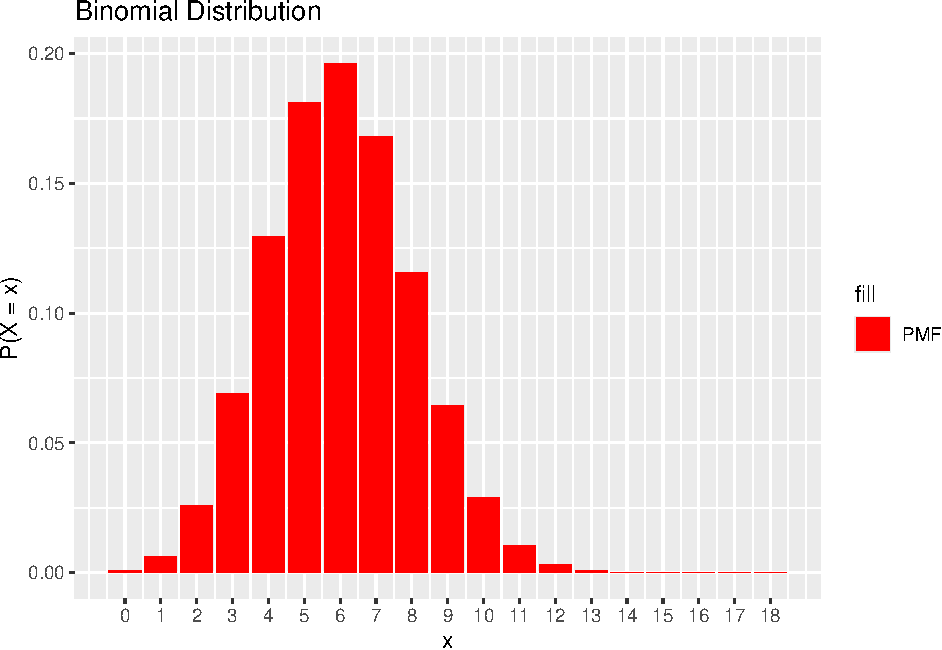
\includegraphics{es_files/figure-latex/unnamed-chunk-5-1.pdf}

\hypertarget{b}{%
\subsection{B}\label{b}}

Plot the Cumulative Distribution Function for the Poisson distribution
with \(\lambda = 3\). Calculate:

\begin{enumerate}
\def\labelenumi{\arabic{enumi}.}
\tightlist
\item
  \(P(X=3)\)
\end{enumerate}

\begin{Shaded}
\begin{Highlighting}[]
\NormalTok{lambda \textless{}{-}}\StringTok{ }\DecValTok{3}
\KeywordTok{dpois}\NormalTok{(}\DecValTok{3}\NormalTok{, lambda)}
\CommentTok{\#\# [1] 0.2240418}
\end{Highlighting}
\end{Shaded}

\begin{enumerate}
\def\labelenumi{\arabic{enumi}.}
\setcounter{enumi}{1}
\tightlist
\item
  \(P(X \ge 3)\)
\end{enumerate}

\begin{Shaded}
\begin{Highlighting}[]
\KeywordTok{ppois}\NormalTok{(}\DecValTok{2}\NormalTok{, lambda, }\DataTypeTok{lower.tail =} \OtherTok{FALSE}\NormalTok{)}
\CommentTok{\#\# [1] 0.5768099}
\end{Highlighting}
\end{Shaded}

\begin{enumerate}
\def\labelenumi{\arabic{enumi}.}
\setcounter{enumi}{2}
\tightlist
\item
  \(P(1 \le X > 5)\)
\end{enumerate}

\begin{Shaded}
\begin{Highlighting}[]
\KeywordTok{ppois}\NormalTok{(}\DecValTok{4}\NormalTok{, lambda) }\OperatorTok{{-}}\StringTok{ }\KeywordTok{ppois}\NormalTok{(}\DecValTok{0}\NormalTok{, lambda)}
\CommentTok{\#\# [1] 0.7654762}
\end{Highlighting}
\end{Shaded}

\begin{enumerate}
\def\labelenumi{\arabic{enumi}.}
\setcounter{enumi}{3}
\tightlist
\item
  \(P(X \ge 15)\)
\end{enumerate}

\begin{Shaded}
\begin{Highlighting}[]
\KeywordTok{ppois}\NormalTok{(}\DecValTok{14}\NormalTok{, lambda, }\DataTypeTok{lower.tail =} \OtherTok{FALSE}\NormalTok{)}
\CommentTok{\#\# [1] 6.703859e{-}07}
\end{Highlighting}
\end{Shaded}

\begin{Shaded}
\begin{Highlighting}[]
\NormalTok{df \textless{}{-}}\StringTok{ }\KeywordTok{data.frame}\NormalTok{(}\DataTypeTok{x =} \DecValTok{0}\OperatorTok{:}\DecValTok{18}\NormalTok{, }\DataTypeTok{y =} \KeywordTok{ppois}\NormalTok{(}\DecValTok{0}\OperatorTok{:}\DecValTok{18}\NormalTok{, lambda))}

\KeywordTok{ggplot}\NormalTok{(df, }\KeywordTok{aes}\NormalTok{(}\DataTypeTok{x =}\NormalTok{ x, }\DataTypeTok{y =}\NormalTok{ y, }\DataTypeTok{color =} \StringTok{"CDF"}\NormalTok{)) }\OperatorTok{+}
\StringTok{  }\KeywordTok{geom\_step}\NormalTok{() }\OperatorTok{+}
\StringTok{  }\KeywordTok{scale\_x\_continuous}\NormalTok{(}\DataTypeTok{breaks =} \DecValTok{0}\OperatorTok{:}\DecValTok{18}\NormalTok{) }\OperatorTok{+}
\StringTok{  }\KeywordTok{scale\_color\_manual}\NormalTok{(}\DataTypeTok{values =} \StringTok{"blue"}\NormalTok{) }\OperatorTok{+}
\StringTok{  }\KeywordTok{labs}\NormalTok{(}
    \DataTypeTok{title =} \StringTok{"Poisson Distribution"}\NormalTok{,}
    \DataTypeTok{x =} \StringTok{"x"}\NormalTok{,}
    \DataTypeTok{y =} \StringTok{"P(X \textless{}= x)"}
\NormalTok{  )}
\end{Highlighting}
\end{Shaded}

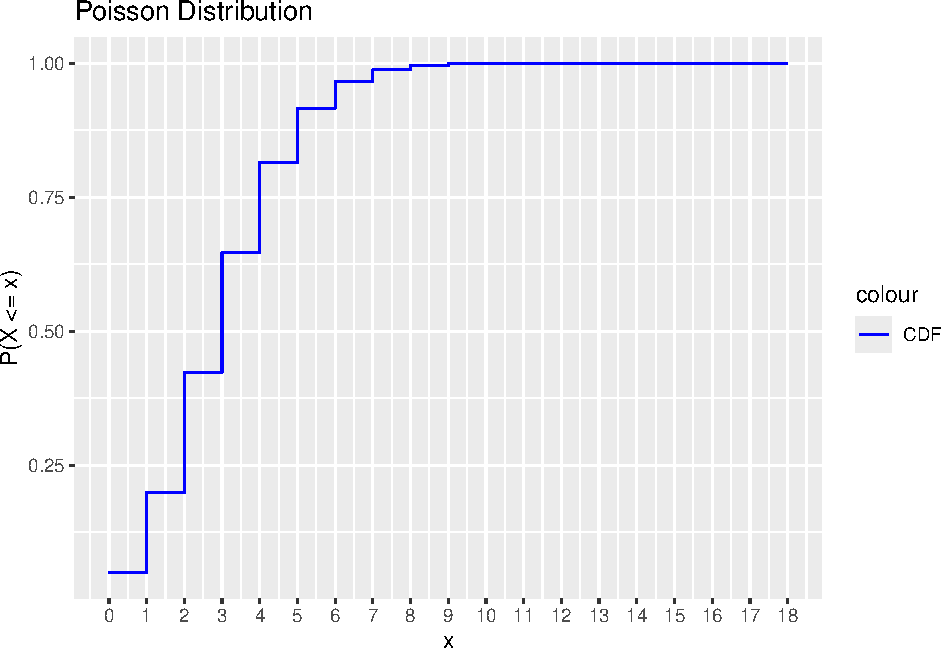
\includegraphics{es_files/figure-latex/unnamed-chunk-10-1.pdf}

\hypertarget{exercise-2}{%
\section{Exercise 2}\label{exercise-2}}

Demonstrate that a Poisson r.v. may be used as an approximation for a
binomial r.v.

\hypertarget{a-1}{%
\subsection{A}\label{a-1}}

\begin{Shaded}
\begin{Highlighting}[]
\NormalTok{n \textless{}{-}}\StringTok{ }\KeywordTok{c}\NormalTok{(}\DecValTok{20}\NormalTok{, }\DecValTok{30}\NormalTok{, }\DecValTok{40}\NormalTok{, }\DecValTok{100}\NormalTok{)}
\NormalTok{p \textless{}{-}}\StringTok{ }\KeywordTok{c}\NormalTok{(}\DecValTok{1} \OperatorTok{/}\StringTok{ }\DecValTok{4}\NormalTok{, }\DecValTok{1} \OperatorTok{/}\StringTok{ }\DecValTok{6}\NormalTok{, }\DecValTok{1} \OperatorTok{/}\StringTok{ }\DecValTok{8}\NormalTok{, }\DecValTok{1} \OperatorTok{/}\StringTok{ }\DecValTok{20}\NormalTok{)}

\NormalTok{pmf \textless{}{-}}\StringTok{ }\KeywordTok{matrix}\NormalTok{(}\OtherTok{NA}\NormalTok{, }\DataTypeTok{nrow =} \DecValTok{21}\NormalTok{, }\DataTypeTok{ncol =} \DecValTok{4}\NormalTok{)}

\ControlFlowTok{for}\NormalTok{ (i }\ControlFlowTok{in} \DecValTok{1}\OperatorTok{:}\DecValTok{4}\NormalTok{) \{}
\NormalTok{  pmf[, i] \textless{}{-}}\StringTok{ }\KeywordTok{dbinom}\NormalTok{(}\DecValTok{0}\OperatorTok{:}\DecValTok{20}\NormalTok{, n[i], p[i])}
\NormalTok{\}}

\NormalTok{pmf \textless{}{-}}\StringTok{ }\KeywordTok{as.data.frame}\NormalTok{(pmf)}

\KeywordTok{colnames}\NormalTok{(pmf) \textless{}{-}}\StringTok{ }\KeywordTok{paste}\NormalTok{(}\StringTok{"Binomial"}\NormalTok{, n, }\KeywordTok{round}\NormalTok{(p, }\DecValTok{2}\NormalTok{), }\DataTypeTok{sep =} \StringTok{"\_"}\NormalTok{)}

\NormalTok{pmf}\OperatorTok{$}\NormalTok{Poisson \textless{}{-}}\StringTok{ }\KeywordTok{dpois}\NormalTok{(}\DecValTok{0}\OperatorTok{:}\DecValTok{20}\NormalTok{, n }\OperatorTok{*}\StringTok{ }\NormalTok{p)}

\NormalTok{pmf}\OperatorTok{$}\NormalTok{X \textless{}{-}}\StringTok{ }\DecValTok{0}\OperatorTok{:}\DecValTok{20}
\end{Highlighting}
\end{Shaded}

\hypertarget{b-1}{%
\subsection{B}\label{b-1}}

\begin{Shaded}
\begin{Highlighting}[]
\KeywordTok{library}\NormalTok{(reshape2)}

\NormalTok{df\_plot \textless{}{-}}\StringTok{ }\KeywordTok{melt}\NormalTok{(pmf, }\DataTypeTok{id.vars =} \StringTok{"X"}\NormalTok{)}
\NormalTok{df\_plot}
\end{Highlighting}
\end{Shaded}

\begin{verbatim}
##      X          variable        value
## 1    0  Binomial_20_0.25 3.171212e-03
## 2    1  Binomial_20_0.25 2.114141e-02
## 3    2  Binomial_20_0.25 6.694781e-02
## 4    3  Binomial_20_0.25 1.338956e-01
## 5    4  Binomial_20_0.25 1.896855e-01
## 6    5  Binomial_20_0.25 2.023312e-01
## 7    6  Binomial_20_0.25 1.686093e-01
## 8    7  Binomial_20_0.25 1.124062e-01
## 9    8  Binomial_20_0.25 6.088669e-02
## 10   9  Binomial_20_0.25 2.706075e-02
## 11  10  Binomial_20_0.25 9.922275e-03
## 12  11  Binomial_20_0.25 3.006750e-03
## 13  12  Binomial_20_0.25 7.516875e-04
## 14  13  Binomial_20_0.25 1.541923e-04
## 15  14  Binomial_20_0.25 2.569872e-05
## 16  15  Binomial_20_0.25 3.426496e-06
## 17  16  Binomial_20_0.25 3.569266e-07
## 18  17  Binomial_20_0.25 2.799425e-08
## 19  18  Binomial_20_0.25 1.555236e-09
## 20  19  Binomial_20_0.25 5.456968e-11
## 21  20  Binomial_20_0.25 9.094947e-13
## 22   0  Binomial_30_0.17 4.212720e-03
## 23   1  Binomial_30_0.17 2.527632e-02
## 24   2  Binomial_30_0.17 7.330133e-02
## 25   3  Binomial_30_0.17 1.368292e-01
## 26   4  Binomial_30_0.17 1.847194e-01
## 27   5  Binomial_30_0.17 1.921081e-01
## 28   6  Binomial_30_0.17 1.600901e-01
## 29   7  Binomial_30_0.17 1.097761e-01
## 30   8  Binomial_30_0.17 6.312124e-02
## 31   9  Binomial_30_0.17 3.085927e-02
## 32  10  Binomial_30_0.17 1.296090e-02
## 33  11  Binomial_30_0.17 4.713053e-03
## 34  12  Binomial_30_0.17 1.492467e-03
## 35  13  Binomial_30_0.17 4.132985e-04
## 36  14  Binomial_30_0.17 1.003725e-04
## 37  15  Binomial_30_0.17 2.141280e-05
## 38  16  Binomial_30_0.17 4.014899e-06
## 39  17  Binomial_30_0.17 6.612776e-07
## 40  18  Binomial_30_0.17 9.551787e-08
## 41  19  Binomial_30_0.17 1.206542e-08
## 42  20  Binomial_30_0.17 1.327196e-09
## 43   0  Binomial_40_0.12 4.789852e-03
## 44   1  Binomial_40_0.12 2.737058e-02
## 45   2  Binomial_40_0.12 7.624663e-02
## 46   3  Binomial_40_0.12 1.379701e-01
## 47   4  Binomial_40_0.12 1.823176e-01
## 48   5  Binomial_40_0.12 1.875267e-01
## 49   6  Binomial_40_0.12 1.562722e-01
## 50   7  Binomial_40_0.12 1.084338e-01
## 51   8  Binomial_40_0.12 6.389849e-02
## 52   9  Binomial_40_0.12 3.245638e-02
## 53  10  Binomial_40_0.12 1.437354e-02
## 54  11  Binomial_40_0.12 5.600080e-03
## 55  12  Binomial_40_0.12 1.933361e-03
## 56  13  Binomial_40_0.12 5.948803e-04
## 57  14  Binomial_40_0.12 1.638956e-04
## 58  15  Binomial_40_0.12 4.058367e-05
## 59  16  Binomial_40_0.12 9.058855e-06
## 60  17  Binomial_40_0.12 1.826996e-06
## 61  18  Binomial_40_0.12 3.334992e-07
## 62  19  Binomial_40_0.12 5.516529e-08
## 63  20  Binomial_40_0.12 8.274793e-09
## 64   0 Binomial_100_0.05 5.920529e-03
## 65   1 Binomial_100_0.05 3.116068e-02
## 66   2 Binomial_100_0.05 8.118177e-02
## 67   3 Binomial_100_0.05 1.395757e-01
## 68   4 Binomial_100_0.05 1.781426e-01
## 69   5 Binomial_100_0.05 1.800178e-01
## 70   6 Binomial_100_0.05 1.500149e-01
## 71   7 Binomial_100_0.05 1.060255e-01
## 72   8 Binomial_100_0.05 6.487089e-02
## 73   9 Binomial_100_0.05 3.490130e-02
## 74  10 Binomial_100_0.05 1.671588e-02
## 75  11 Binomial_100_0.05 7.198228e-03
## 76  12 Binomial_100_0.05 2.809834e-03
## 77  13 Binomial_100_0.05 1.001075e-03
## 78  14 Binomial_100_0.05 3.274191e-04
## 79  15 Binomial_100_0.05 9.880016e-05
## 80  16 Binomial_100_0.05 2.762505e-05
## 81  17 Binomial_100_0.05 7.184222e-06
## 82  18 Binomial_100_0.05 1.743539e-06
## 83  19 Binomial_100_0.05 3.960394e-07
## 84  20 Binomial_100_0.05 8.441893e-08
## 85   0           Poisson 6.737947e-03
## 86   1           Poisson 3.368973e-02
## 87   2           Poisson 8.422434e-02
## 88   3           Poisson 1.403739e-01
## 89   4           Poisson 1.754674e-01
## 90   5           Poisson 1.754674e-01
## 91   6           Poisson 1.462228e-01
## 92   7           Poisson 1.044449e-01
## 93   8           Poisson 6.527804e-02
## 94   9           Poisson 3.626558e-02
## 95  10           Poisson 1.813279e-02
## 96  11           Poisson 8.242177e-03
## 97  12           Poisson 3.434240e-03
## 98  13           Poisson 1.320862e-03
## 99  14           Poisson 4.717363e-04
## 100 15           Poisson 1.572454e-04
## 101 16           Poisson 4.913920e-05
## 102 17           Poisson 1.445271e-05
## 103 18           Poisson 4.014640e-06
## 104 19           Poisson 1.056484e-06
## 105 20           Poisson 2.641211e-07
\end{verbatim}

\begin{Shaded}
\begin{Highlighting}[]
\KeywordTok{library}\NormalTok{(ggplot2)}
\KeywordTok{library}\NormalTok{(RColorBrewer) }\CommentTok{\# Color palettes}

\KeywordTok{ggplot}\NormalTok{(df\_plot, }\KeywordTok{aes}\NormalTok{(}\DataTypeTok{x =}\NormalTok{ X, }\DataTypeTok{y =}\NormalTok{ value, }\DataTypeTok{color =}\NormalTok{ variable)) }\OperatorTok{+}
\StringTok{  }\KeywordTok{geom\_line}\NormalTok{() }\OperatorTok{+}
\StringTok{  }\KeywordTok{scale\_color\_manual}\NormalTok{(}\DataTypeTok{values =} \KeywordTok{c}\NormalTok{(}\KeywordTok{brewer.pal}\NormalTok{(}\DecValTok{4}\NormalTok{, }\StringTok{"PRGn"}\NormalTok{), }\StringTok{"red"}\NormalTok{)) }\OperatorTok{+}
\StringTok{  }\KeywordTok{labs}\NormalTok{(}
    \DataTypeTok{title =} \StringTok{"Binomial vs Poisson PMF"}\NormalTok{,}
    \DataTypeTok{x =} \StringTok{"x"}\NormalTok{,}
    \DataTypeTok{y =} \StringTok{"P(X = x)"}
\NormalTok{  )}
\end{Highlighting}
\end{Shaded}

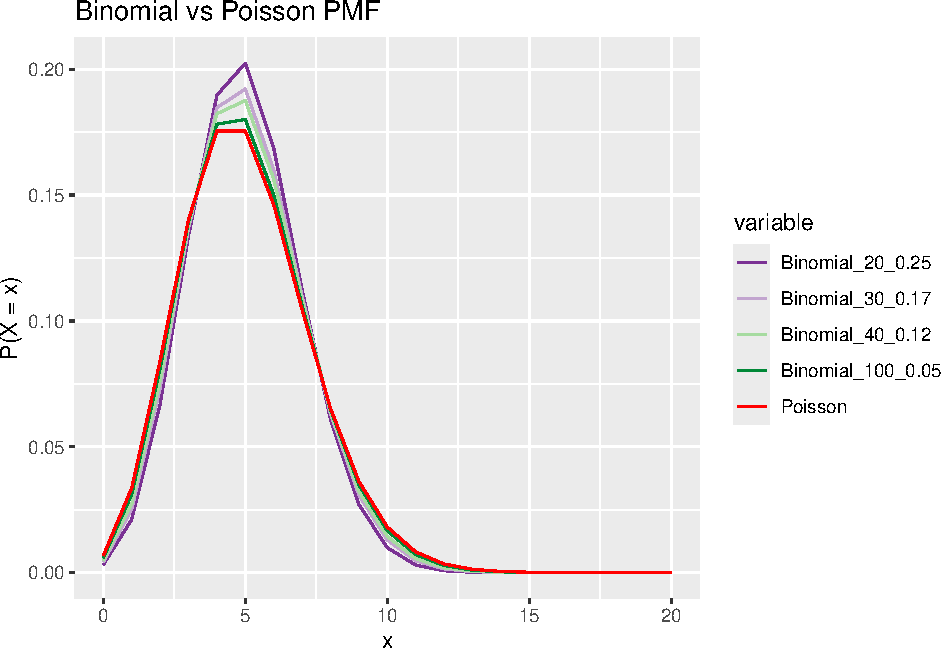
\includegraphics{es_files/figure-latex/unnamed-chunk-12-1.pdf}

\hypertarget{exercise-3}{%
\section{Exercise 3}\label{exercise-3}}

\hypertarget{a-2}{%
\subsection{A}\label{a-2}}

Generate N=1000 random numbers from a binomial distribution with n=9
trials and p=0.8. Thus each of the 1000 random numbers will be an
integer between 0 and 9.

\begin{Shaded}
\begin{Highlighting}[]
\KeywordTok{set.seed}\NormalTok{(}\DecValTok{123}\NormalTok{)}
\NormalTok{n \textless{}{-}}\StringTok{ }\DecValTok{9}
\NormalTok{p \textless{}{-}}\StringTok{ }\FloatTok{0.8}
\NormalTok{t \textless{}{-}}\StringTok{ }\DecValTok{1000}

\NormalTok{valori \textless{}{-}}\StringTok{ }\KeywordTok{rbinom}\NormalTok{(t, n, p)}
\end{Highlighting}
\end{Shaded}

\hypertarget{b-2}{%
\subsection{B}\label{b-2}}

Plot the experimental probability using the geom\_bar() function.

\begin{Shaded}
\begin{Highlighting}[]
\NormalTok{df \textless{}{-}}\StringTok{ }\KeywordTok{data.frame}\NormalTok{(}\DataTypeTok{x =}\NormalTok{ valori)}

\KeywordTok{ggplot}\NormalTok{(df, }\KeywordTok{aes}\NormalTok{(}\DataTypeTok{x =}\NormalTok{ valori)) }\OperatorTok{+}
\StringTok{  }\KeywordTok{geom\_bar}\NormalTok{() }\OperatorTok{+}
\StringTok{  }\KeywordTok{scale\_x\_continuous}\NormalTok{(}\DataTypeTok{breaks =} \DecValTok{0}\OperatorTok{:}\DecValTok{9}\NormalTok{) }\OperatorTok{+}
\StringTok{  }\KeywordTok{labs}\NormalTok{(}
    \DataTypeTok{title =} \StringTok{"Experimental Probability"}\NormalTok{,}
    \DataTypeTok{x =} \StringTok{"Successes"}\NormalTok{,}
    \DataTypeTok{y =} \StringTok{"Frequency"}
\NormalTok{  )}
\end{Highlighting}
\end{Shaded}

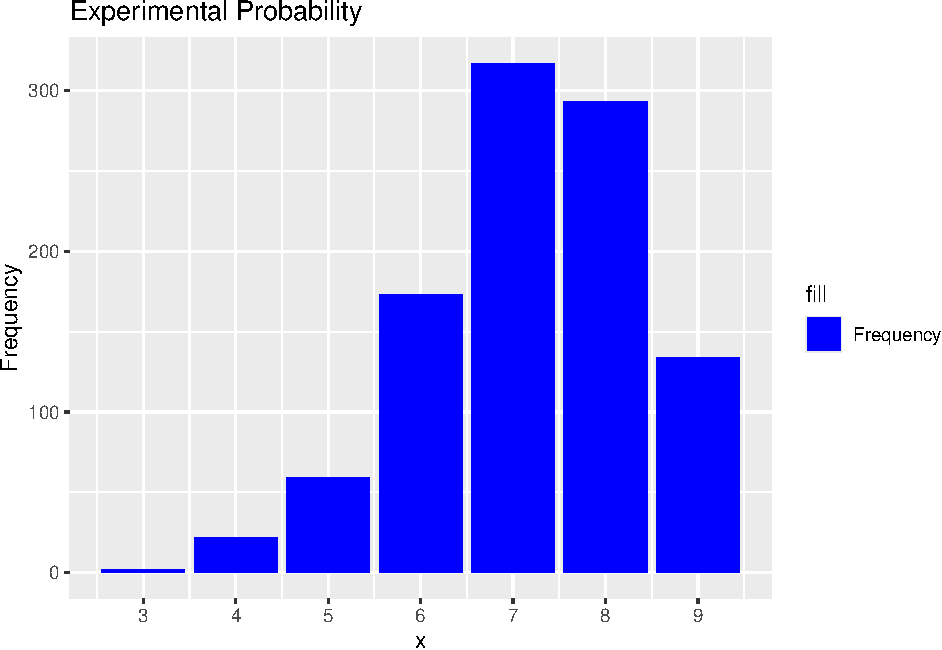
\includegraphics{es_files/figure-latex/unnamed-chunk-14-1.pdf}

\hypertarget{c}{%
\subsection{C}\label{c}}

For each value of the x-axis obtained in the previous plot, compute the
real probability mass function and add it in the plot as red dots using
geom\_point().

\begin{Shaded}
\begin{Highlighting}[]
\NormalTok{p\_teo \textless{}{-}}\StringTok{ }\KeywordTok{data.frame}\NormalTok{(}\DataTypeTok{p =} \KeywordTok{dbinom}\NormalTok{(}\DecValTok{0}\OperatorTok{:}\DecValTok{9}\NormalTok{, n, p))}

\KeywordTok{ggplot}\NormalTok{(df, }\KeywordTok{aes}\NormalTok{(}\DataTypeTok{x =}\NormalTok{ valori)) }\OperatorTok{+}
\StringTok{  }\KeywordTok{geom\_bar}\NormalTok{(}\KeywordTok{aes}\NormalTok{(}\DataTypeTok{y =} \KeywordTok{after\_stat}\NormalTok{(prop))) }\OperatorTok{+}
\StringTok{  }\KeywordTok{geom\_point}\NormalTok{(}
    \DataTypeTok{data =}\NormalTok{ p\_teo,}
    \KeywordTok{aes}\NormalTok{(}
      \DataTypeTok{x =} \DecValTok{0}\OperatorTok{:}\DecValTok{9}\NormalTok{, }\DataTypeTok{y =}\NormalTok{ p,}
      \DataTypeTok{color =} \StringTok{"red"}
\NormalTok{    ),}
\NormalTok{  ) }\OperatorTok{+}
\StringTok{  }\KeywordTok{scale\_x\_continuous}\NormalTok{(}\DataTypeTok{breaks =} \DecValTok{0}\OperatorTok{:}\DecValTok{9}\NormalTok{) }\OperatorTok{+}
\StringTok{  }\KeywordTok{labs}\NormalTok{(}
    \DataTypeTok{title =} \StringTok{"Experimental vs Real Probability"}\NormalTok{,}
    \DataTypeTok{x =} \StringTok{"Successes"}\NormalTok{,}
    \DataTypeTok{y =} \StringTok{"Frequency"}
\NormalTok{  )}
\end{Highlighting}
\end{Shaded}

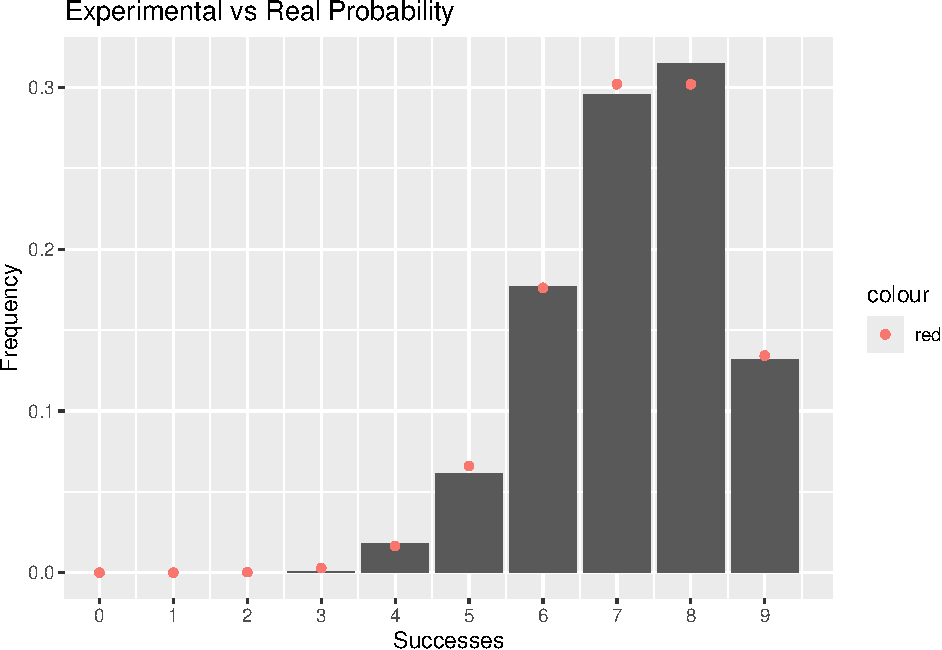
\includegraphics{es_files/figure-latex/unnamed-chunk-15-1.pdf}

\hypertarget{exercise-4}{%
\section{Exercise 4}\label{exercise-4}}

Suppose the number of customers visiting a retail store follows a
Poisson distribution with a mean of 5 customers per hour. (hint:
\(X \sim Poisson(\lambda=5)\))

Find the probability that in a randomely chosen hour, there will be:

\hypertarget{a-3}{%
\subsection{A}\label{a-3}}

No customers

\begin{Shaded}
\begin{Highlighting}[]
\NormalTok{lambda \textless{}{-}}\StringTok{ }\DecValTok{5}
\KeywordTok{dpois}\NormalTok{(}\DecValTok{0}\NormalTok{, lambda)}
\end{Highlighting}
\end{Shaded}

\begin{verbatim}
## [1] 0.006737947
\end{verbatim}

\hypertarget{b-3}{%
\subsection{B}\label{b-3}}

At least 3 customers

\begin{Shaded}
\begin{Highlighting}[]
\KeywordTok{ppois}\NormalTok{(}\DecValTok{2}\NormalTok{, lambda, }\DataTypeTok{lower.tail =} \OtherTok{FALSE}\NormalTok{)}
\end{Highlighting}
\end{Shaded}

\begin{verbatim}
## [1] 0.875348
\end{verbatim}

\hypertarget{c-1}{%
\subsection{C}\label{c-1}}

Exactly 7 customers

\begin{Shaded}
\begin{Highlighting}[]
\KeywordTok{dpois}\NormalTok{(}\DecValTok{7}\NormalTok{, lambda)}
\end{Highlighting}
\end{Shaded}

\begin{verbatim}
## [1] 0.1044449
\end{verbatim}

\hypertarget{d}{%
\subsection{D}\label{d}}

Assuming that each customer buys something that costs a price from 10€
to 50€. Which is the expected value of a customer expense? (hint: Y =
customer expense \textasciitilde{} Uniform(10, 50))

\begin{Shaded}
\begin{Highlighting}[]
\NormalTok{a \textless{}{-}}\StringTok{ }\DecValTok{10}
\NormalTok{b \textless{}{-}}\StringTok{ }\DecValTok{50}

\NormalTok{e\_y \textless{}{-}}\StringTok{ }\NormalTok{(a }\OperatorTok{+}\StringTok{ }\NormalTok{b) }\OperatorTok{/}\StringTok{ }\DecValTok{2}
\NormalTok{e\_y}
\end{Highlighting}
\end{Shaded}

\begin{verbatim}
## [1] 30
\end{verbatim}

\hypertarget{e}{%
\subsection{E}\label{e}}

How many customers are expected in 8 working hours?

\begin{Shaded}
\begin{Highlighting}[]
\NormalTok{h \textless{}{-}}\StringTok{ }\DecValTok{8}

\NormalTok{e\_x \textless{}{-}}\StringTok{ }\NormalTok{lambda }\OperatorTok{*}\StringTok{ }\NormalTok{h}
\NormalTok{e\_x}
\end{Highlighting}
\end{Shaded}

\begin{verbatim}
## [1] 40
\end{verbatim}

\hypertarget{f}{%
\subsection{F}\label{f}}

Using rpois() and runif() functions, simulate the customers and their
expenses in a normal day made of 8 working hours. Represent the data as
similar as possible to the plot below (hints: prepare a data.frame
containing as many rows as the number of customers of the entire day.
For each customer, store its ID number, the hour, and the money he/she
spent. Use facet\_grid with scales = ``free\_x''. Search on google how
to do the rest).

\begin{Shaded}
\begin{Highlighting}[]
\NormalTok{t \textless{}{-}}\StringTok{ }\DecValTok{5}
\NormalTok{h \textless{}{-}}\StringTok{ }\DecValTok{8}

\KeywordTok{set.seed}\NormalTok{(}\DecValTok{123}\NormalTok{)}
\NormalTok{customers \textless{}{-}}\StringTok{ }\KeywordTok{rpois}\NormalTok{(h }\OperatorTok{*}\StringTok{ }\NormalTok{t, lambda)}
\NormalTok{expenses \textless{}{-}}\StringTok{ }\KeywordTok{runif}\NormalTok{(t, }\DecValTok{10}\NormalTok{, }\DecValTok{50}\NormalTok{)}

\NormalTok{df \textless{}{-}}\StringTok{ }\KeywordTok{data.frame}\NormalTok{(}
  \DataTypeTok{customer =} \KeywordTok{rep}\NormalTok{(}\DecValTok{1}\OperatorTok{:}\NormalTok{t, }\DataTypeTok{each =}\NormalTok{ h),}
  \DataTypeTok{hour =} \KeywordTok{rep}\NormalTok{(}\DecValTok{1}\OperatorTok{:}\NormalTok{h, t),}
  \DataTypeTok{expense =}\NormalTok{ expenses}
\NormalTok{)}

\CommentTok{\# Plot each hour in a separate facet}
\KeywordTok{ggplot}\NormalTok{(df, }\KeywordTok{aes}\NormalTok{(}\DataTypeTok{x =}\NormalTok{ customer, }\DataTypeTok{y =}\NormalTok{ expense)) }\OperatorTok{+}
\StringTok{  }\KeywordTok{geom\_col}\NormalTok{() }\OperatorTok{+}
\StringTok{  }\KeywordTok{facet\_grid}\NormalTok{(}\OperatorTok{\textasciitilde{}}\NormalTok{hour, }\DataTypeTok{scales =} \StringTok{"free\_x"}\NormalTok{) }\OperatorTok{+}
\StringTok{  }\KeywordTok{labs}\NormalTok{(}
    \DataTypeTok{title =} \StringTok{"Customer Expenses"}\NormalTok{,}
    \DataTypeTok{x =} \StringTok{"Customer ID"}\NormalTok{,}
    \DataTypeTok{y =} \StringTok{"Expense"}
\NormalTok{  ) }\OperatorTok{+}
\StringTok{  }\KeywordTok{theme\_minimal}\NormalTok{()}
\end{Highlighting}
\end{Shaded}

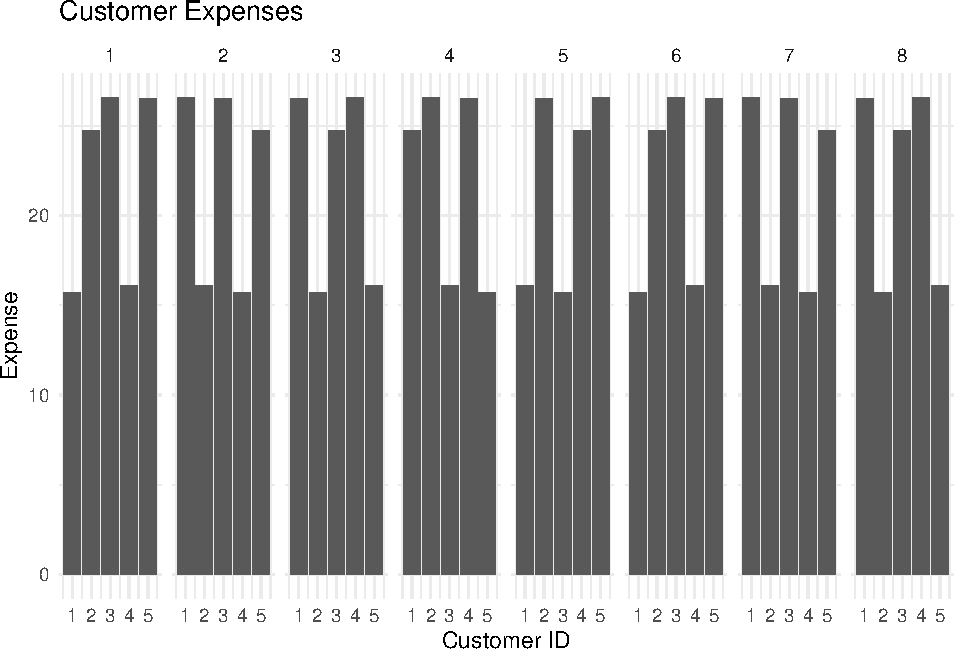
\includegraphics{es_files/figure-latex/unnamed-chunk-21-1.pdf}

\hypertarget{exercise-5}{%
\section{Exercise 5}\label{exercise-5}}

In a survey of a sample of 500 university students, they were asked if
they know how to program in R. The collected data showed that 240
students know how to program in R. Consider the discrete random variable
X, which indicates the number of students in a random sample of 50
students who know how to program in R.

\hypertarget{a-4}{%
\subsection{A}\label{a-4}}

Compute the probability mass function of X and draw a plot.

\begin{Shaded}
\begin{Highlighting}[]
\NormalTok{students \textless{}{-}}\StringTok{ }\DecValTok{500}
\NormalTok{know\_r \textless{}{-}}\StringTok{ }\DecValTok{240}
\NormalTok{sample\_size \textless{}{-}}\StringTok{ }\DecValTok{50}

\KeywordTok{dhyper}\NormalTok{(}\DecValTok{0}\OperatorTok{:}\DecValTok{50}\NormalTok{, students, students }\OperatorTok{{-}}\StringTok{ }\NormalTok{know\_r, sample\_size)}
\end{Highlighting}
\end{Shaded}

\begin{verbatim}
##  [1] 1.712717e-25 2.029286e-23 1.170237e-21 4.377677e-20 1.194605e-18
##  [6] 2.535451e-17 4.357806e-16 6.235766e-15 7.579816e-14 7.946693e-13
## [11] 7.271586e-12 5.862735e-11 4.197005e-10 2.684693e-09 1.542586e-08
## [16] 7.996764e-08 3.754012e-07 1.600830e-06 6.217258e-06 2.203976e-05
## [21] 7.144235e-05 2.120738e-04 5.771781e-04 1.441491e-03 3.305727e-03
## [26] 6.963691e-03 1.347683e-02 2.395881e-02 3.911283e-02 5.859870e-02
## [31] 8.049996e-02 1.012849e-01 1.165483e-01 1.224346e-01 1.171659e-01
## [36] 1.018762e-01 8.023788e-02 5.703308e-02 3.642637e-02 2.079578e-02
## [41] 1.054554e-02 4.713777e-03 1.839816e-03 6.196420e-04 1.773653e-04
## [46] 4.228946e-05 8.169881e-06 1.228289e-06 1.347904e-07 9.601336e-09
## [51] 3.330925e-10
\end{verbatim}

\begin{Shaded}
\begin{Highlighting}[]
\NormalTok{df \textless{}{-}}\StringTok{ }\KeywordTok{data.frame}\NormalTok{(}\DataTypeTok{x =} \DecValTok{20}\OperatorTok{:}\DecValTok{44}\NormalTok{, }\DataTypeTok{y =} \KeywordTok{dhyper}\NormalTok{(}
  \DecValTok{20}\OperatorTok{:}\DecValTok{44}\NormalTok{,}
\NormalTok{  students,}
\NormalTok{  students }\OperatorTok{{-}}\StringTok{ }\NormalTok{know\_r,}
\NormalTok{  sample\_size}
\NormalTok{))}

\KeywordTok{ggplot}\NormalTok{(df, }\KeywordTok{aes}\NormalTok{(}\DataTypeTok{x =}\NormalTok{ x, }\DataTypeTok{y =}\NormalTok{ y)) }\OperatorTok{+}
\StringTok{  }\KeywordTok{geom\_col}\NormalTok{() }\OperatorTok{+}
\StringTok{  }\KeywordTok{scale\_x\_continuous}\NormalTok{(}\DataTypeTok{breaks =} \DecValTok{0}\OperatorTok{:}\DecValTok{50}\NormalTok{) }\OperatorTok{+}
\StringTok{  }\KeywordTok{labs}\NormalTok{(}
    \DataTypeTok{title =} \StringTok{"Hypergeometric Distribution"}\NormalTok{,}
    \DataTypeTok{x =} \StringTok{"x"}\NormalTok{,}
    \DataTypeTok{y =} \StringTok{"P(X = x)"}
\NormalTok{  ) }\OperatorTok{+}
\StringTok{  }\KeywordTok{theme\_minimal}\NormalTok{()}
\end{Highlighting}
\end{Shaded}

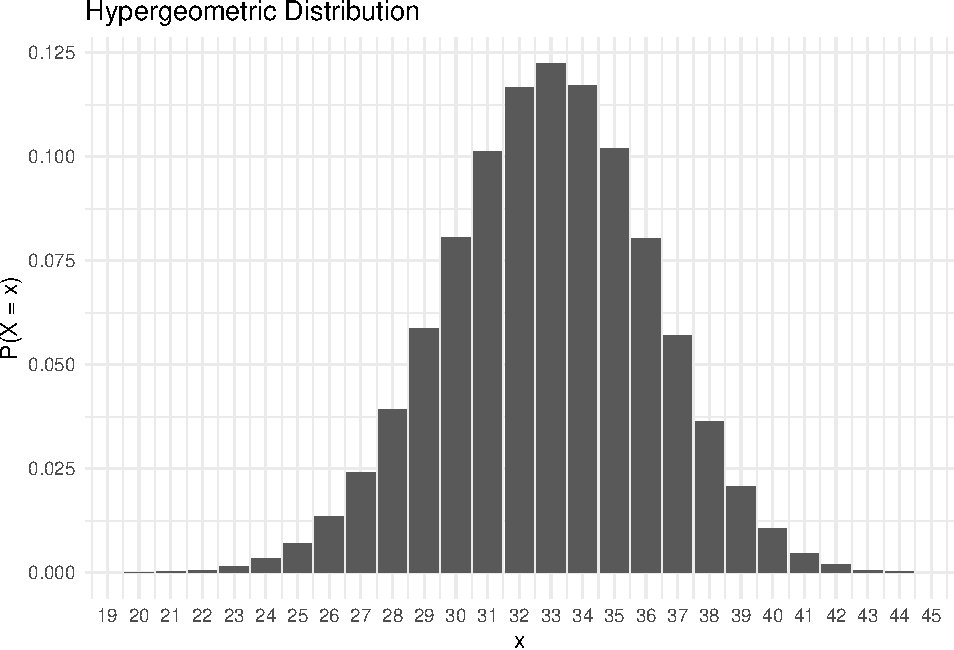
\includegraphics{es_files/figure-latex/unnamed-chunk-22-1.pdf}

\hypertarget{b-4}{%
\subsection{B}\label{b-4}}

Calculate the probability that at least 30 students in the sample of 50
know how to program in R.

\begin{Shaded}
\begin{Highlighting}[]
\DecValTok{1} \OperatorTok{{-}}\StringTok{ }\KeywordTok{phyper}\NormalTok{(}\DecValTok{29}\NormalTok{, students, students }\OperatorTok{{-}}\StringTok{ }\NormalTok{know\_r, sample\_size)}
\end{Highlighting}
\end{Shaded}

\begin{verbatim}
## [1] 0.8522509
\end{verbatim}

\hypertarget{c-2}{%
\subsection{C}\label{c-2}}

Calculate the expected value of X.

\begin{Shaded}
\begin{Highlighting}[]
\NormalTok{students }\OperatorTok{*}\StringTok{ }\NormalTok{sample\_size }\OperatorTok{/}\StringTok{ }\NormalTok{students}
\end{Highlighting}
\end{Shaded}

\begin{verbatim}
## [1] 50
\end{verbatim}

\end{document}
